% A LaTeX template for MSc Thesis submissions to 
% Politecnico di Milano (PoliMi) - School of Industrial and Information Engineering
%
% S. Bonetti, A. Gruttadauria, G. Mescolini, A. Zingaro
% e-mail: template-tesi-ingind@polimi.it
%
% Last Revision: October 2021
%
% Copyright 2021 Politecnico di Milano, Italy. NC-BY

\documentclass{Configuration_Files/PoliMi3i_thesis}

%------------------------------------------------------------------------------
%	REQUIRED PACKAGES AND  CONFIGURATIONS
%------------------------------------------------------------------------------

% CONFIGURATIONS
\usepackage{parskip} % For paragraph layout
\usepackage{setspace} % For using single or double spacing
\usepackage{emptypage} % To insert empty pages
\usepackage{multicol} % To write in multiple columns (executive summary)
\setlength\columnsep{15pt} % Column separation in executive summary
\setlength\parindent{0pt} % Indentation
\raggedbottom  

% PACKAGES FOR TITLES
\usepackage{titlesec}
% \titlespacing{\section}{left spacing}{before spacing}{after spacing}
\titlespacing{\section}{0pt}{3.3ex}{2ex}
\titlespacing{\subsection}{0pt}{3.3ex}{1.65ex}
\titlespacing{\subsubsection}{0pt}{3.3ex}{1ex}
\usepackage{color}

% PACKAGES FOR LANGUAGE AND FONT
\usepackage[english]{babel} % The document is in English  
\usepackage[utf8]{inputenc} % UTF8 encoding
\usepackage[T1]{fontenc} % Font encoding
\usepackage[11pt]{moresize} % Big fonts

% PACKAGES FOR IMAGES
\usepackage{graphicx}
\usepackage{transparent} % Enables transparent images
\usepackage{eso-pic} % For the background picture on the title page
\usepackage{subfig} % Numbered and caption subfigures using \subfloat.
\usepackage{tikz} % A package for high-quality hand-made figures.
\usetikzlibrary{}
\graphicspath{{./Images/}} % Directory of the images
\usepackage{caption} % Coloured captions
\usepackage{xcolor} % Coloured captions
\usepackage{amsthm,thmtools,xcolor} % Coloured "Theorem"
\usepackage{float}

% STANDARD MATH PACKAGES
\usepackage{amsmath}
\usepackage{amsthm}
\usepackage{amssymb}
\usepackage{amsfonts}
\usepackage{bm}
\usepackage[overload]{empheq} % For braced-style systems of equations.
\usepackage{fix-cm} % To override original LaTeX restrictions on sizes

% PACKAGES FOR TABLES
\usepackage{tabularx}
\usepackage{longtable} % Tables that can span several pages
\usepackage{colortbl}

% PACKAGES FOR ALGORITHMS (PSEUDO-CODE)
\usepackage{algorithm}
\usepackage{algpseudocode}
% PACKAGES FOR REFERENCES & BIBLIOGRAPHY
\usepackage[backend=biber]{biblatex} %Imports biblatex package, specify biber backend
\addbibresource{mimesis.bib}
% PACKAGES FOR REFERENCES & BIBLIOGRAPHY
\usepackage[colorlinks=true,linkcolor=black,anchorcolor=black,citecolor=black,filecolor=black,menucolor=black,runcolor=black,urlcolor=black]{hyperref} % Adds clickable links at references
\usepackage{cleveref}

% OTHER PACKAGES
\usepackage{pdfpages} % To include a pdf file
\usepackage{afterpage}
\usepackage{lipsum} % DUMMY PACKAGE
\usepackage{fancyhdr} % For the headers
\fancyhf{}

% Input of configuration file. Do not change config.tex file unless you really know what you are doing. 


% Create color bluePoli (-> manuale grafica coordinata:  https://www.polimi.it/fileadmin/user_upload/il_Politecnico/grafica-coordinata/2015_05_11_46xy_manuale_grafica_coordinata.pdf)
\definecolor{bluePoli}{cmyk}{0.4,0.1,0,0.4}

% Custom theorem environments
\declaretheoremstyle[
  shaded={rulecolor=bluePoli!20, rulewidth=1pt, bgcolor=bluePoli!5},
  headfont=\color{bluePoli}\normalfont\bfseries,
  bodyfont=\color{black}\normalfont,
]{colored}

\captionsetup[figure]{labelfont={color=bluePoli}} % Set colour of the captions
\captionsetup[table]{labelfont={color=bluePoli}} % Set colour of the captions
\captionsetup[algorithm]{labelfont={color=bluePoli}} % Set colour of the captions

% \theoremstyle{colored}
% \newtheorem{theorem}{Theorem}[section]
% \newtheorem{proposition}{Proposition}[section]
% \newtheorem{definition}{Definition}[section]
% \newtheorem*{remark}{Remark}
% \newtheorem{lemma}{Lemma}[section]



%----------------------------------------------------------------------------
%	NEW COMMANDS DEFINED
%----------------------------------------------------------------------------

% EXAMPLES OF NEW COMMANDS
\newcommand{\bea}{\begin{eqnarray}} % Shortcut for equation arrays
\newcommand{\eea}{\end{eqnarray}}
\newcommand{\e}[1]{\times 10^{#1}}  % Powers of 10 notation

%----------------------------------------------------------------------------
%	ADD YOUR PACKAGES (be careful of package interaction)
%----------------------------------------------------------------------------

%----------------------------------------------------------------------------
%	ADD YOUR DEFINITIONS AND COMMANDS (be careful of existing commands)
%----------------------------------------------------------------------------
\newcommand*{\oldepsilon}{\epsilon}
\renewcommand*{\epsilon}{\varepsilon}
\DeclareMathOperator*{\esssup}{ess\,sup}
\DeclareMathOperator*{\argmax}{arg\,max}
\DeclareMathOperator*{\argmin}{arg\,min}
%----------------------------------------------------------------------------
%	BEGIN OF YOUR DOCUMENT
%----------------------------------------------------------------------------

\begin{document}

\fancypagestyle{plain}{%
\fancyhf{} % Clear all header and footer fields
\fancyhead[RO,RE]{\thepage} %RO=right odd, RE=right even
\renewcommand{\headrulewidth}{0pt}
\renewcommand{\footrulewidth}{0pt}}

%----------------------------------------------------------------------------
%	TITLE PAGE
%----------------------------------------------------------------------------

\pagestyle{empty} % No page numbers
\frontmatter % Use roman page numbering style (i, ii, iii, iv...) for the preamble pages

\puttitle{
	title=Neural Modes, % Title of the thesis
	name=Andrea Bonifacio, % Author Name and Surname
	course=Mathematical Engineering - Ingegneria Matematica, % Study Programme (in Italian)
	ID  = 217658,  % Student ID number (numero di matricola)
	advisor= Prof. Stefano Pagani, % Supervisor name
	coadvisor={Stéphane Cotin}, % Co-Supervisor name, remove this line if there is none
	academicyear={2024-25},  % Academic Year
} % These info will be put into your Title page 

%----------------------------------------------------------------------------
%	PREAMBLE PAGES: ABSTRACT (inglese e italiano), EXECUTIVE SUMMARY
%----------------------------------------------------------------------------
\startpreamble
\setcounter{page}{1} % Set page counter to 1

% ABSTRACT IN ENGLISH
\chapter*{Abstract} 
Here goes the Abstract in English of your thesis followed by a list of keywords.
The Abstract is a concise summary of the content of the thesis (single page of text)
and a guide to the most important contributions included in your thesis.
The Abstract is the very last thing you write.
It should be a self-contained text and should be clear to someone who hasn't (yet) read the whole manuscript.
The Abstract should contain the answers to the main scientific questions that have been addressed in your thesis.
It needs to summarize the adopted motivations and the adopted methodological approach as well as the findings of your work and their relevance and impact.
The Abstract is the part appearing in the record of your thesis inside POLITesi,
the Digital Archive of PhD and Master Theses (Laurea Magistrale) of Politecnico di Milano.
The Abstract will be followed by a list of four to six keywords.
Keywords are a tool to help indexers and search engines to find relevant documents.
To be relevant and effective, keywords must be chosen carefully.
They should represent the content of your work and be specific to your field or sub-field.
Keywords may be a single word or two to four words. 
\\
\\
\textbf{Keywords:} here, the keywords, of your thesis % Keywords

% ABSTRACT IN ITALIAN
\chapter*{Abstract in lingua italiana}
Qui va l'Abstract in lingua italiana della tesi seguito dalla lista di parole chiave.
\\
\\
\textbf{Parole chiave:} qui, vanno, le parole chiave, della tesi % Keywords (italian)

%----------------------------------------------------------------------------
%	LIST OF CONTENTS/FIGURES/TABLES/SYMBOLS
%----------------------------------------------------------------------------

% TABLE OF CONTENTS
\thispagestyle{empty}
\tableofcontents % Table of contents 
\thispagestyle{empty}
\cleardoublepage

%-------------------------------------------------------------------------
%	THESIS MAIN TEXT
%-------------------------------------------------------------------------
% In the main text of your thesis you can write the chapters in two different ways:
%
%(1) As presented in this template you can write:
%    \chapter{Title of the chapter}
%    *body of the chapter*
%
%(2) You can write your chapter in a separated .tex file and then include it in the main file with the following command:
%    \chapter{Title of the chapter}
%    \input{chapter_file.tex}
%
% Especially for long thesis, we recommend you the second option.

\addtocontents{toc}{\vspace{2em}} % Add a gap in the Contents, for aesthetics
\mainmatter % Begin numeric (1,2,3...) page numbering

% --------------------------------------------------------------------------
% NUMBERED CHAPTERS % Regular chapters following
% --------------------------------------------------------------------------
\chapter*{Introduction}
\section{Introduction}

Numerical simulations play a critical role in a wide array of scientific and engineering applications, providing insights into the behavior of physical systems under various conditions. Among the most prominent techniques for performing such simulations is Finite Element Modeling (FEM). FEM discretizes a continuous domain into a mesh of finite elements, allowing for the approximation of solutions to complex partial differential equations (PDEs). However, one significant drawback of FEM is its computational intensity, especially when high resolution is required for accurate results. This research aims to explore the potential of Deep Learning (DL) techniques to accelerate FEM simulations, focusing specifically on the deformation of objects subjected to external forces.

The deformation of an object under an applied force is directly tied to the object's discretization. In FEM, the object is represented by a mesh, where the resolution of the mesh—i.e., the size and number of elements—clearly impacts the accuracy and computational cost of the simulation. High-resolution meshes can capture fine details of deformation, leading to more accurate simulations, but they are computationally expensive and time-consuming. 

The main goal of this work is to study the efficacy of a method that combines both Finite Element Modeling (FEM) and DL to obtain a realistic simulation of an object in a fraction of the time that would be required by a traditional FEM simulation. The idea is to, somehow, train a DL model to have inside the information given by the refined discretization and pass them on a coarser discretization.

The idea of using DL techniques to solve scientific problem is not new. Thanks to the rise of new frameworks and libraries, such as TensorFlow and PyTorch, it is now possible to train very complex models on large datasets in a reasonable amount of time. For the problem at hand, a lot of different approaches can be found in the existing literature: a lot of them are based on the idea that the deep learning model should predict the whole dynamic of the system, for example MeshGraphNet \cite{pfaffLearningMeshBasedSimulation2021a} or its multiscale version \cite{fortunatoMultiScaleMeshGraphNets2022}, but these are just two examples of the many possible approaches \cite{jiangMeshfreeFlowNetPhysicsConstrainedDeep2020}, \cite{djeumouNeuralNetworksPhysicsInformed2022}, \cite{hanPredictingPhysicsMeshreduced2022a}. Other methods rely on solving a time independent problem, using various architectures, such as PINNs \cite{djeumouNeuralNetworksPhysicsInformed2022} or GNNs \cite{gaoPhysicsinformedGraphNeural2022}. The proposed method falls into the second category, as it will be explained in the following sections.

The inspiration for this work came from the world of Computational Fluid Dynamics (CFD), particularly from a paper in which the authors propose a data-driven correction to the solution of a coarse grid simulation, using a neural network trained on the fine grid simulation \cite{kienerDatadrivenCorrectionCoarse2023}. The main concept is to create two grids on a fixed domain in a way that the fine grid is a refinement of the coarse grid. In this way, by means of an interpolation operator, it is possible to have both solutions on the same grid and perform computations with them, such as the difference between the two solution or between the derivatives of the solution. The neural network is trained to predict the difference between the fine grid solution and the coarse grid solution, given the coarse grid solution as input. In the paper, they propose various machine learning models, such as a simple feedforward neural network, a random forest and a GNN, both in two and three dimensions. The results show that the neural network is able to predict the difference between the two solutions with a good accuracy. 

This work aims at finding a solution to the problem of accelerating FEM simulations in the context of solid mechanics. To achieve such a goal, a good method should have certain characteristics: \begin{itemize}
    \item It should be geometry independent, removing the need for a new training for each new geometry.ù
    \item Should at least be topology independent, meaning that the method should be able to work with different meshes.
    \item Avoid the ``black-box'' problem of having a model predict the whole system without having any insights on what's happening inside.
    \item It should be really fast, to be able to be used in real-time applications.
\end{itemize}
Of those, the first one is clearly the most difficult to achieve, as encoding a geometry is still an open problem. Some progress were made in the field CITARE GINO, but it's far from solved. Also, for the uses of this method, it is assumed that the geometry is known, so this problem is not addressed here. 

The other three points are addressed here. Let's start by the independence with respect to the topology. In the original paper, the authors found a way to superimpose the two grids, but that would imply that the two meshes must be created together, limiting the possibilities. In this case it is possible to take advantage of the FEM itself, allowing to compute the exact solution everywhere on the domain, and then interpolate it on the mutual grid. By following this approach, it is possible to have a method that is independent of the topology of the mesh, since the position of the points on the grid is always the same with respect to the domain.

The main problem with ``black-box'' models is that they are not interpretable, so if the model isn't working as expected, it is difficult to understand why. One example is the MeshGraphNet, which is a very complex model that tries to fully predict the dynamic of the system. If the prediction is accumulating errors, one must retrain the model from scratch, trying to understand what went wrong. In this case, the method is based on correcting a numerical solution, so the starting point is always the exact solution which the model is trained to correct, so theoretically should be easier to understand the weaknesses of the model.

Finally, the speed of the method is a critical point. The method should be able to be used in real-time applications, so it should be as fast as possible. The method proposed here is based on a neural network, which means that instead of solving a linear system of equations, the solution is obtained by a forward pass of the network, which basically consists of a series of matrix multiplications and non-linear functions. This is a very fast operation, especially if the network is small, so the method should be able to be used in real-time applications.

The rest of the report is organized as follows: Section \ref{sec:problem_setting} introduces the problem setting and the mathematical formulation of the problem. Section \ref{sec:neural_network} gives a brief overview of the neural network architectures used in this work. Section \ref{sec:numerical_results} presents the numerical results obtained by the proposed method on selected tests. Finally, Section \ref{sec:conclusions} summarizes the main findings and outlines possible future research directions.

\chapter{Mathematical Model}
\label{ch:chapter_one}%
\section{Mathematical Framework}
\label{sec:problem_setting}

Simulating the dynamic behavior of soft tissues is crucial in various applications, from surgical planning to biomechanical analysis. However, accurately capturing the complex, nonlinear deformations of these materials remains a significant computational challenge. In this section, we present our mathematical framework for addressing this challenge. Our approach is made up of three core elements: a hyperelastic mechanical model to represent the material's constitutive behavior, linear modal analysis for efficient dimensionality reduction, and a novel neural modes technique to incorporate nonlinear effects. By integrating these elements, we aim to achieve accurate and computationally lighter simulations of soft tissue deformation.


\subsection{Mechanical Model}
\label{sec:mechanical_model}

To model the deformation of an object, we start from the vector \(\bm{X}\), which represents the material coordinates in the reference configuration (i.e. its non-deformed state). Any deformation of the object can be described by the displacement vector \(\bm{u}(\bm{X},t)\), which maps the material coordinates to the spatial coordinates \(\bm{x}\) in the deformed configuration. The relationship between these two configurations is given by:
\begin{equation}
    \bm{x}(\bm{X},t) = \bm{X} + \bm{u}(\bm{X},t),
\label{eq:deformation}
\end{equation}
where \(\bm{x} \in \mathbb{R}^d\) is the spatial position of a material point at time \(t\), and \(d\) is the spatial dimension (2D or 3D). 

To model the mechanical behavior of the material, there are many constitutive models available, ranging from linear elastic to hyperelastic models \cite{Ogden_1997}. Since we are interested in soft tissue mechanics, we will focus on the hyperelastic Neo-Hookean material model \cite{Ogden_1997}. Such a model helps dealing with large deformations and is suitable for biological tissues, which often exhibit nonlinear elastic behavior.
More complex hyperelastic models exist, such as the Mooney-Rivlin or Ogden models \cite{Ogden_1997}, which can provide greater accuracy for specific materials or loading conditions, but at the cost of increased computational complexity and parameter identification.

For the Neo-Hookean hyperelastic material model, we first compute the deformation gradient $\bm{F} \in \mathbb{R}^{d\times d}$:
\begin{equation}
    \bm{F} = \frac{\partial \bm{x}}{\partial \bm{X}} = \bm{I} + \nabla_{\mathbf{X}} \bm{u},
\label{eq:deformation_gradient}
\end{equation}
where $\bm{I} \in \mathbb{R}^{d\times d}$ is the identity matrix and $\nabla_{\mathbf{X}}$ denotes the gradient with respect to material coordinates. The right Cauchy-Green deformation tensor is then defined as $\bm{C} = \bm{F}^T\bm{F}$, and the first invariant of $\bm{C}$ is $I_{\bm{C}} = \text{tr}(\bm{C})$.

The Neo-Hookean strain-energy density function $\Psi$ is given by:
\begin{equation}
    \Psi(\bm{F}) = \frac{\mu}{2} (I_C - 3 - 2\ln(J)) + \frac{\lambda}{4} (J^2 - 1 - 2\ln(J)),
\label{eq:neo_hookean_energy}
\end{equation}
where $J = \det(\bm{F})$ is the determinant of the deformation gradient (representing the volume change ratio), $\mu$ is the shear modulus, and $\lambda$ is the first Lamé parameter. These material parameters are related to the Young's modulus $E$ and the Poisson's ratio $\nu$ by:
\begin{equation}
    \mu = \frac{E}{2(1+\nu)} \quad \text{and} \quad \lambda = \frac{E\nu}{(1+\nu)(1-2\nu)}.
\end{equation}

From the strain energy density function, we derive the first Piola-Kirchhoff stress tensor $\bm{P}$:
\begin{equation}
    \bm{P} = \frac{\partial \Psi}{\partial \bm{F}} = \mu \bm{F} - \mu \bm{F}^{-T} + \frac{\lambda}{2}(J^2-1)\bm{F}^{-T}.
\label{eq:piola_stress}
\end{equation}

For static problems the equation of equilibrium is given by:
\begin{equation}
    \begin{cases}
        - \nabla_X \cdot \bm{P} = \bm{b} \quad \text{in} \quad \Omega, \\
        \bm{u} = \bm{u}_D \quad \text{on} \quad \Gamma_D, \\
        \bm{P} \cdot \bm{N} = \bm{t} \quad \text{on} \quad \Gamma_N.
    \end{cases}
\label{eq:static_problem}
\end{equation}
This represents a boundary value problem that needs to be solved for the displacement field $\bm{u}$, where $\Omega$ is the domain of interest, $\Gamma_D$ is the Dirichlet boundary where displacements are prescribed, and $\Gamma_N$ is the Neumann boundary where tractions are applied. The vector $\bm{b}$ represents external body forces, and $\bm{t}$ is the traction applied on the boundary. The unit normal vector $\bm{N}$ is defined on the boundary $\Gamma_N$.

For dynamic problems, the equation of motion including inertial forces is:
\begin{equation}
    \begin{cases}
        \rho \frac{\partial^2 \bm{u}}{\partial t^2} - \nabla_X \cdot \bm{P} = \bm{b} \quad \text{in} \quad \Omega, \\
        \bm{u} = \bm{u}_D \quad \text{on} \quad \Gamma_D, \\
        \bm{P} \cdot \bm{N} = \bm{t} \quad \text{on} \quad \Gamma_N,
    \end{cases}
\label{eq:dynamic_problem}
\end{equation}
where $\rho$ is the material density in the reference configuration and the rest follows the same notation as in the static case. 
The weak form of equation \eqref{eq:dynamic_problem} is:
\begin{equation}
    \int_{\Omega} \rho \frac{\partial^2 \bm{u}}{\partial t^2} \cdot \bm{v} \, d\Omega + \int_{\Omega} \bm{P} : \nabla_X \bm{v} \, d\Omega = \int_{\Omega} \bm{b} \cdot \bm{v} \, d\Omega + \int_{\Gamma_N} \bm{t} \cdot \bm{v} \, d\Gamma,
\label{eq:weak_form}
\end{equation}
where $\bm{v} \in \{\bm{v} \in H^1(\Omega) | \bm{v} = \bm{0} \text{ on } \Gamma_D\}$ is any vector-valued test function with $H^1(\Omega)$ being a Hilbert space. 

\subsection{Linear Modal Analysis}
\label{sec:linear_modes}

Simulating the deformation of mechanical objects in real-time poses significant computational challenges. A common technique to accelerate these simulations, particularly in computer graphics and computational mechanics, is modal analysis \cite{Pentland_Williams_1989}. This approach leverages the idea that the complex deformation of an object can often be well-approximated by a combination of its dominant, low-frequency vibration patterns, known as modes. The modal analysis technique allows us to reduce the dimensionality of the problem by focusing on these low-frequency modes, thus enabling faster simulations while maintaining a reasonable level of accuracy.


The core steps of linear modal analysis are as follows:

\begin{enumerate}
    \item \textbf{Linearize the System}: The first step involves linearizing the governing equations around the undeformed state ($\bm{u}=\bm{0}$). This results in a constant stiffness matrix $\bm{K}$ and a mass matrix $\bm{M}$. The mass matrix $\bm{M}$ captures the inertial properties of the system:
        \begin{equation}
            \bm{M} = \int_{\Omega} \rho \bm{\phi}^T \bm{\phi} \, d\Omega, 
            \label{eq:mass_matrix}
        \end{equation}
        where $\bm{\phi}$ represents the shape functions used in the finite element discretization, while the stiffness matrix $\bm{K}$ represents the system's resistance to small deformations around the rest state and is derived from the linearization of the internal forces (i.e., the derivative of the internal force vector with respect to displacement, evaluated at $\bm{u}=\bm{0}$). For a hyperelastic material like Neo-Hookean, this linearization effectively corresponds to the standard linear elastic stiffness matrix at the origin.

    \item \textbf{Solve the Generalized Eigenvalue Problem}: With the linearized system matrices, we solve the generalized eigenvalue problem:
        \begin{equation}
            \bm{K} \bm{\phi}_i = \omega_i^2 \bm{M} \bm{\phi}_i.
            \label{eq:eigenvalue_problem}
        \end{equation}
        Here, $\omega_i^2$ are the eigenvalues, representing the squared natural frequencies of vibration, and $\bm{\phi}_i$ are the corresponding eigenvectors, representing the spatial shapes of these vibration modes (mode shapes). The modes are typically ordered by increasing frequency.

    \item \textbf{Modal Decomposition}: A reduced basis is formed by selecting the first $m$ modes (eigenvectors), typically those corresponding to the lowest frequencies, which capture the large-scale deformations. The displacement field $\bm{u}(\bm{X},t)$ can then be approximated as a linear combination of these modes:
        \begin{equation}
            \bm{u}(\bm{X},t) \approx \sum_{i=1}^{m} z_i(t) \bm{\phi}_i(\bm{X}),
            \label{eq:modal_decomposition}
        \end{equation}
        where $z_i(t)$ are the time-varying modal coordinates, representing the amplitude or contribution of each mode shape to the overall deformation. The dynamics of the system can then be simulated in the reduced $m$-dimensional space of modal coordinates, significantly reducing computational cost.
\end{enumerate}

While linear modal analysis provides substantial speedups, its fundamental limitation lies in the initial linearization, done in the first step of this process. This approximation holds well only for small deformations around the rest state. Indeed, when deformations become large and enter the nonlinear regime characteristic of hyperelastic materials like Neo-Hookean, the linear modal approximation breaks down. Specifically, the constant stiffness matrix $\bm{K}$ no longer accurately represents the material's resistance to deformation. It fails to capture the nonlinear effects accurately, often leading to unrealistic behavior such as exaggerated volume changes or inaccurate stress distributions.



\chapter{Chapter two}
\label{ch:chapter_two}%
\section{Methods}
\label{sec:methods}

This section details the computational methodologies employed to learn and utilize nonlinear deformation modes, addressing the challenges of simulating complex soft tissue behavior. We begin by laying the groundwork with a review of fundamental neural network concepts, which are central to our data-driven learning strategy. Following this, we explore the principles of subspace learning, demonstrating how neural networks can be trained to efficiently represent solutions to constrained physical problems. The core of our proposed method, the 'Neural Modes' architecture, is then introduced, including its specific design and the physics-informed loss functions crucial for its training. Finally, we describe the integration of these learned modes into dynamic simulations and discuss potential avenues for extending the framework's capabilities.



\subsection{Neural Network Principles}

A Neural Network (NN) is a mathematical model that achieves statistical generalization drawing inspiration from the human brain. Indeed, it is based on neurons, which are connected one to another, and carry the information from the input to the output.

It is possible to define NN as a function that maps an input to an output, given a set of parameters \( \bm{\theta} \). The function \( \hat{y} = f(\bm{x}; \bm{\theta}) \) is obtained by composing a series of functions \( f_i \) called layers, where each layer is defined as
\begin{equation}
    f_i = \sigma(W_i f_{i-1} + b_i),
\end{equation}
where \( W_i \) is the weight matrix, \( b_i \) is the bias vector and \( \sigma(\cdot) \) is the activation function. The activation function is a non-linear function that allows the network to learn complex patterns in the data. 

A neural network is trained using a dataset \( \mathcal{D} = \{(\bm{x}_i, \bm{y}_i)\}_{i=1}^N \), where \( \bm{x}_i \) is the input and \( \bm{y}_i \) is the corresponding target output. The objective is to find the optimal set of parameters \( \bm{\theta} \) that minimizes a loss function \( \mathcal{L} \), which quantifies the discrepancy between the network's predictions and the true outputs. The loss function is defined as:
\begin{equation}
    \mathcal{L}(\bm{\theta}) = \frac{1}{N} \sum_{i=1}^N L(f(\bm{x}_i; \bm{\theta}), \bm{y}_i)
\end{equation}
where \( L \) is a per-sample loss function (e.g., Mean Squared Error). The optimization process aims to find the parameters \( \bm{\theta}^* \) that minimize the overall loss:
\begin{equation}
    \bm{\theta}^* = \argmin_{\bm{\theta}} \mathcal{L}(\bm{\theta}).
\end{equation}
Common optimization algorithms include Gradient Descent, Adam, and L-BFGS \cite{Liu_1989}.

The full algorithm is the following one:
\begin{algorithm} 
    \caption{Training of a neural network}
    \begin{algorithmic}
        \State Initialize the parameters \( \bm{\theta} \)
        \While{epoch < max\_epochs}
            \For{mini-batch in dataset}
                \State Perform forward pass computing \( f(\bm{x}; \bm{\theta}) \)
                \State Compute the loss function \( \mathcal{L}(f(\bm{x}; \bm{\theta}), \bm{y}) \)
                \State Perform backward pass computing the gradients of the loss function
                \State Update the parameters using the gradients
            \EndFor
        \EndWhile
    \end{algorithmic}
\end{algorithm}



\subsection{Neural Network Architectures}
In this work, we employ a deep residual neural network specifically designed for learning nonlinear deformation modes. This architecture builds upon traditional fully connected neural networks but incorporates residual connections to facilitate the training of deeper networks and improve performance in capturing nonlinear corrections to linear modal displacements.


\subsubsection{Neural Modes Architecture}
The Neural Modes architecture is designed to learn nonlinear corrections to linear deformation modes for Neo-Hookean materials. It consists of a deep residual neural network. The architecture is defined as follows:

\begin{itemize}
    \item The input is a modal coordinate vector \( \bm{z} \in \mathbb{R}^m \), where $m$ is the number of modal coordinates. These modal coordinates represent the weights of the linear modes used to approximate the deformation.
    \item The network consists of several residual blocks, each containing two fully connected layers with Leaky ReLU activation functions, and a skip connection that adds the input of the block to its output. The number of residual blocks and the number of neurons per layer are hyperparameters that can be tuned to optimize performance.
    \item The output layer has a linear activation function and outputs a nonlinear correction to the displacement field \( \bm{y} \in \mathbb{R}^n \), where $n$ is the total number of degrees of freedom in the mesh. This correction is added to the linear modal displacement to obtain a more accurate approximation of the deformed configuration.
\end{itemize}

The network learns to map from the reduced modal space to full-dimensional correction vectors that improve the accuracy of the linear modal approximation. This architecture, which we call Neural Modes, can be visualized as a mapping from a low-dimensional modal space to a high-dimensional displacement space, where the neural network learns to correct the linear approximation provided by the modal basis. The following figure illustrates the architecture:
% H per bloccare la figura. altrimenti metti la referenza
\begin{figure}[H] 
    \centering
    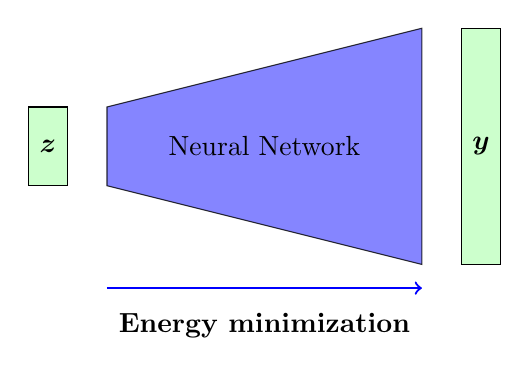
\begin{tikzpicture}
        % Modal coordinate (z)
        \draw[fill=green!20] (-3, 1) rectangle (-2.5,2);
        \node at (-2.75, 1.5) {$\bm{z}$}; % Label inside the rectangle
        
        % Displacement (u)
        \draw[fill=green!20] (2.5,0) rectangle (3,3);
        \node at (2.75, 1.5) {$\bm{y}$}; % Label inside the rectangle
        
        % Energy loss transition
        \draw[fill=blue!60,opacity=0.8] (-2,1) -- (2,-0) -- (2,3) -- (-2,2) -- cycle;
        \node at (0,1.5) {Neural Network};
        \node[below] at (0,-0.5) {\textbf{Energy minimization}};
        
        % Energy loss arrow
        \draw[thick,blue,->] (-2,-0.3) -- (2,-0.3);
    
    \end{tikzpicture}
    \caption{Neural Modes architecture for learning nonlinear deformation corrections}
    \label{fig:neural_modes_arch}
\end{figure}



\subsubsection{Training the Neural Modes}
The training process for the Neural Modes Network is based on minimizing a combination of physics-based losses, rather than simply minimizing the prediction error against ground truth data, which is the classical loss used in most neural network training. The key terms that build the loss used in training are:

\begin{enumerate}
    \item \textbf{Energy Loss}: minimizes the internal strain energy of the deformed configuration $E(\bm{X} + \bm{l} + \bm{y})$, where $\bm{X}$ is the rest position, $\bm{l}$ is the linear mode displacement given by $\bm{z}$, and $\bm{y}$ is the nonlinear correction.
    
    \item \textbf{Orthogonality Loss}: ensures that the nonlinear correction is orthogonal to the linear mode space: $\bm{y}^T \bm{l} = 0$.

    \item \textbf{Boundary Condition Penalty}: enforces the displacement boundary conditions on the deformed configuration.
    
\end{enumerate}

The total loss function is a weighted sum of these individual losses:
\begin{equation}
    \text{Loss} = \text{Energy Loss} + \lambda_1 \text{Orthogonality Loss} + \lambda_2 \text{Boundary Condition Penalty},
\end{equation}
where $\lambda_1$ and $\lambda_2$ are weight parameters that balance the importance of each loss term.

During the training process, we observed that the network tended to learn a non-zero correction even when the input modal coordinate vector was zero (\(\bm{z} = \bm{0}\)), corresponding to the rest position. Ideally, the network's output should be zero at the rest position, indicating no deformation correction. Unlike \cite{Wang_Du_Coros_Thomaszewski_2024}, who address this issue by adding an explicit origin loss term to their loss function, we enforce a zero correction at the origin by using a bias-free neural network architecture. This design choice ensures that the network's output is naturally centered around zero, promoting a zero correction when no modal displacement is applied.

During training, the Neural Modes network is optimized using a self-supervised learning approach, where the loss function is designed to minimize the internal energy of the deformed configuration while enforcing orthogonality and boundary condition constraints. Specifically, we employ the Adam optimizer to minimize a loss function that combines the energy loss with penalty terms for deviations from orthogonality and boundary conditions. The per-sample loss function \( L \) includes a Mean Squared Error (MSE) term for each constraint, ensuring that deviations are quadratically penalized. This approach allows the network to learn the underlying physics of the deformation without relying on precomputed ground truth data.


\subsection{Subspace Learning}
\begin{align}
    \label{eq:constrained_energy_minimization}
    \bm{x}^*(\phi, \psi) = \underset{\bm{x}}{\argmin} \quad & E_\phi(\bm{x}) \\
    \text{s.t.} \quad & C_\psi(\bm{x}) = 0, \nonumber
\end{align}
where \( E_\phi \) is the energy function defined by parameters \(\phi\) and \( C_\psi \) is the constraint function with parameters \(\psi\). The solution set \( \bm{x}^*\) constitutes a subspace of the full-dimensional space \( \mathbb{R}^d \). In a classical Finite Element framework, sampling from this subspace is achieved by solving a constrained minimization problem for each configuration. 

Clearly, this approach is computationally expensive, so we need a more efficient way to sample from the subspace.

The idea proposed by \cite{Wang_Du_Coros_Thomaszewski_2024} is to find a Neural Network \( \bm{x}[\theta^*](\phi, \psi) \) that approximates the solution \( \bm{x}^* \), meaning that the problem becomes:
\begin{align*}
    \bm{x}[\theta^*](\phi, \psi) \approx \underset{\theta}{\argmin} \quad & E_\phi(\bm{x}[\theta](\phi, \psi)) \\
    \text{s.t.} \quad & C_\psi(\bm{x}[\theta](\phi, \psi)) = 0.
\end{align*}

Now, defining the nonlinear modes as 
\begin{align}
    \bm{n}(\bm{z}) = \bm{l} + \argmin_{\bm{y}} \quad & E_\phi(\bm{X} + \bm{l} + \bm{y}) \\ 
    \text{s.t.} \quad & \bm{l}^T \bm{y} = 0,
\end{align}
where \( \bm{l} \) is the linear mode displacement obtained as
\begin{equation}
    \bm{l} = \sum_{i=1}^m z_i \bm{e}_i,
\end{equation}
where \( \bm{e}_i \) is the $i$-th linear mode and \( z_i \) is the corresponding modal coordinate, we can rewrite the problem \ref{eq:constrained_energy_minimization} as:
\begin{align*}
    \bm{n}[\theta^*](\bm{z}) &= \bm{l} + \bm{y}[\theta^*](\bm{z}), \\
    \theta^* = \underset{\theta}{\argmin} \quad & E_\phi(\bm{X} + \bm{l} + \bm{y}[\theta](\bm{z})) \\
    \text{s.t.} \quad & \bm{l}^T \bm{y}[\theta](\bm{z}) = 0.
\end{align*}

Now we define a suitable function that will serve as a loss function for the self-supervised training of the neural network. The loss function is defined as:
\begin{equation}
    \mathcal{L}(\theta) = \mathbb{E}_{\bm{z}} \left[ E(\bm{X} + \bm{l} + \bm{y}[\theta](\bm{z})) + \lambda_1 \bm{l}^T \bm{y}[\theta](\bm{z}) + \lambda_2 \text{B. C. Penalty} \right],
\end{equation}
where \( \lambda_1 \) and \( \lambda_2 \) are hyperparameters that control the importance of the orthogonality and boundary condition penalty terms, respectively. The first term is the energy loss, which minimizes the internal strain energy of the deformed configuration, while the second term ensures that the nonlinear correction is orthogonal to the linear mode space. The third term enforces the displacement boundary conditions on the deformed configuration.

\subsection{Sampling the Modal Space}
One of the main challenges for this method is finding a good way to sample the \(z\) vector that will be used as input for the neural network. Here are two examples that shows how choosing randomly the \(z\) vector can lead to unrealistic results. 
\begin{figure}[H]
    \centering
    \includegraphics[width=0.4\textwidth]{Images/z_random.png}
    \caption{Example of a bad sampling of the modal space, the reference shape is the light blue outline.}
    \label{fig:bad_sampling}
\end{figure}
In this example, the random \(z\) vector has large values in its latter components. These components represent higher-frequency deformation modes, which naturally contain more strain energy. Using these modes with high amplitudes often creates physically unrealistic or extreme configurations. This shows why random sampling across all components of \(z\) can lead to unrealistic deformations.

A better sampling approach considers the physical meaning of each mode. The first components of \(z\) typically correspond to lower-frequency, global deformation modes that represent major shape changes with less energy. Later components represent higher-frequency, localized, and more energetic modes. 

For more effective sampling of the modal space, we can implement a strategic approach to generating the \(z\) vectors. This approach involves assigning larger coefficient values to the first several components of the vector, which typically correspond to the fundamental, lower-frequency deformation modes, while progressively reducing the magnitude of values assigned to later components. By structuring our sampling in this manner, the resulting deformations tend to be significantly more physically realistic and energetically feasible in real-world scenarios. This methodical sampling focuses the neural network's training process on common, naturally occurring deformation patterns rather than directing computational resources toward unlikely, high-energy configurations that rarely manifest in practical applications.

The fundamental issue with purely random sampling across all modal coordinates is that it inadvertently forces the neural network to attempt energy minimization for physically implausible states. Given that the energy landscape for soft tissue deformation is already inherently complex and high-dimensional, introducing this additional unnecessary complexity substantially increases the difficulty of the training process and potentially compromises the quality of the learned model. This consideration underscores the necessity for developing a more sophisticated and physically-informed strategy to efficiently sample the modal space, allowing the network to concentrate on learning the most relevant aspects of the deformation behavior.


\subsection{Dynamic Simulation with Neural Modes}
For dynamic simulations, the Neural Modes framework solves an optimization problem at each time step. Given the current and previous displacement states $\bm{u}_n$ and $\bm{u}_{n-1}$, the modal coordinates for the next time step $\bm{z}_{n+1}$ are computed by:
\begin{equation}
    \bm{z}_{n+1} = \underset{\bm{z}}{\argmin} \frac{1}{2h^2} \|\bm{n}(\bm{z}) - 2\bm{u}_n + \bm{u}_{n-1}\|_{\bm{M}}^2 + E(\bm{n}(\bm{z})),
\end{equation}
where $\bm{n}(\bm{z})$ represents the complete displacement field (linear modes plus nonlinear correction), $h$ is the time step, $\bm{M}$ is the mass matrix, and $E(\cdot)$ is the internal energy of the configuration. This optimization problem is typically solved using the L-BFGS-B algorithm \cite{Liu_1989}.

One challenge with this approach is that the optimization problem does not explicitly account for external forces. The network learns to minimize internal energy but lacks direct information about external forces that may be applied during simulation: this limitation can affect the accuracy of dynamic simulations, particularly for large deformations or complex loading conditions.







\chapter*{Acknowledgements}

\section{Use of copyrighted material}

Each student is responsible for obtaining copyright permissions, if necessary, to include published material in the thesis.
This applies typically to third-party material published by someone else.

\section{Plagiarism}

You have to be sure to respect the rules on Copyright and avoid an involuntary plagiarism.
It is allowed to take other persons' ideas only if the author and his original work are clearly mentioned.
As stated in the Code of Ethics and Conduct, Politecnico di Milano \textit{promotes the integrity of research,
condemns manipulation and the infringement of intellectual property}, and gives opportunity to all those
who carry out research activities to have an adequate training on ethical conduct and integrity while doing research.
To be sure to respect the copyright rules, read the guides on Copyright legislation and citation styles available
at:
\begin{verbatim}
https://www.biblio.polimi.it/en/tools/courses-and-tutorials
\end{verbatim}
You can also attend the courses which are periodically organized on "Bibliographic citations and bibliography management".

\section{Bibliography and citations}
Your thesis must contain a suitable Bibliography which lists all the sources consulted on developing the work.
The list of references is placed at the end of the manuscript after the chapter containing the conclusions.
We suggest to use the BibTeX package and save the bibliographic references  in the file \verb|Thesis_bibliography.bib|.
This is indeed a database containing all the information about the references. To cite in your manuscript, use the \verb|\cite{}| command as follows:
\\
\textit{Here is how you cite bibliography entries: \cite{knuth74}, or multiple ones at once: \cite{knuth92,lamport94}}.
\\
The bibliography and list of references are generated automatically by running BibTeX \cite{bibtex}.

\chapter{Conclusions and future developments}
\label{ch:conclusions}%
A final chapter containing the main conclusions of your research/study
and possible future developments of your work have to be inserted in this chapter.

%-------------------------------------------------------------------------
%	BIBLIOGRAPHY
%-------------------------------------------------------------------------

\addtocontents{toc}{\vspace{2em}} % Add a gap in the Contents, for aesthetics

%-------------------------------------------------------------------------
%	APPENDICES
%-------------------------------------------------------------------------

\cleardoublepage
\addtocontents{toc}{\vspace{2em}} % Add a gap in the Contents, for aesthetics
\appendix
\chapter{Appendix A}
If you need to include an appendix to support the research in your thesis, you can place it at the end of the manuscript.
An appendix contains supplementary material (figures, tables, data, codes, mathematical proofs, surveys, \dots)
which supplement the main results contained in the previous chapters.

\chapter{Appendix B}
It may be necessary to include another appendix to better organize the presentation of supplementary material.


% LIST OF FIGURES
\listoffigures

% LIST OF TABLES
\listoftables

% LIST OF SYMBOLS
% Write out the List of Symbols in this page
\chapter*{List of Symbols} % You have to include a chapter for your list of symbols (
\begin{table}[H]
    \centering
    \begin{tabular}{lll}
        \textbf{Variable} & \textbf{Description} & \textbf{SI unit} \\\hline\\[-9px]
        $\bm{u}$ & solid displacement & m \\[2px]
        $\bm{u}_f$ & fluid displacement & m \\[2px]
    \end{tabular}
\end{table}

% ACKNOWLEDGEMENTS
\chapter*{Acknowledgements}
Here you might want to acknowledge someone.

\cleardoublepage

\end{document}
